At each of the sixteen circles in the network below stands a student. A total of 3360 coins are distributed among the sixteen students. All at once, all students give away all their coins by passing an equal number of coins to each of their neighbors in the network. After the trade, all students have the same number of coins as they started with. Find the number of coins the student standing at the center circle had originally.

\begin{center}
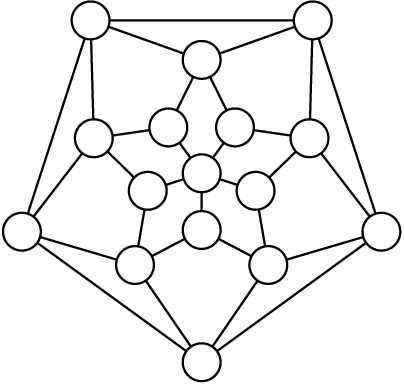
\includegraphics[width = 40.400000000000006mm]{img/fig0.png}
\end{center}